\chapter{Medical Background}

In this chapter, relevant background information from medicine is presented. 

\section{Anatomy of the central nervous system}
The central nervous system (CNS) constits of two parts: the brain and the spinal cord. The CNS receives and process information from all parts of the body. Consequently, studies on the CNS are crucial for our understanding of the human anatomy.
\begin{figure}
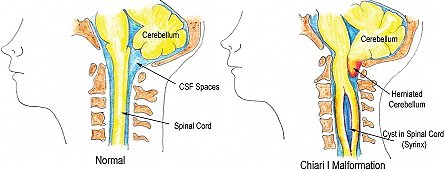
\includegraphics[scale=0.8]{figures/Ida_CSF.png}
\caption{hei}
\end{figure}
\\
\section{The Spinal Cord}


